%%%%%%%%%%%%%%%%%%%%%%%%%%%%%%%%%%%%%%%%%%%%%%%%%%%%%%%%%%%%%%%%%%%%%
%% I, the copyright holder of this work, release this work into the
%% public domain. This applies worldwide. In some countries this may
%% not be legally possible; if so: I grant anyone the right to use
%% this work for any purpose, without any conditions, unless such
%% conditions are required by law.
%%%%%%%%%%%%%%%%%%%%%%%%%%%%%%%%%%%%%%%%%%%%%%%%%%%%%%%%%%%%%%%%%%%%

\documentclass[
  printed, %% This option enables the default options for the
           %% digital version of a document. Replace with `printed`
           %% to enable the default options for the printed version
           %% of a document. printed/digital
  table,   %% Causes the coloring of tables. Replace with `notable`
           %% to restore plain tables.
  nolof,     %% Prints the List of Figures. Replace with `nolof` to
           %% hide the List of Figures.
  nolot, twoside, color
       %% Prints the List of Tables. Replace with `nolot` to
           %% hide the List of Tables.
  %% More options are listed in the user guide at
  %% <http://mirrors.ctan.org/macros/latex/contrib/fithesis/guide/mu/fi.pdf>.
]{fithesis3}
%% The following section sets up the locales used in the thesis.
\usepackage[resetfonts]{cmap} %% We need to load the T2A font encoding
\usepackage[T1,T2A]{fontenc}  %% to use the Cyrillic fonts with Russian texts.
\usepackage[slovak]{babel}        %% foreign texts to be typeset as follows:

%%
%% The following section sets up the metadata of the thesis.
\thesissetup{
    date          = \the\year/\the\month/\the\day,
    university    = mu,
    faculty       = fi,
    type          = mgr,
    author        = Martin Styk,
    gender        = m,
    advisor       = {Ing. Mgr. et Mgr. Zdeněk Říha, Ph.D.},
    title         = {TODO},
    keywords      = {APK súbor, Android, malvér, analýza aplikácií, AndroidManifest.xml},
}
\thesislong{abstract}{
    Táto diplomová práca sa zameriava na detekciu prebalených aplikácií na platforme Android. Cieľom práce je vytvoriť systém detekcie prebalených aplikácií. V rámci práce je vytvorená mobilná aplikácia pre systém Android, ktorá analyzuje nainštalované aplikačné balíčky z ktorých získava detailné metadáta. 
Práca obsahuje návrh a implementáciu metódy detekcie prebalených aplikácií. Algoritmus detekcie využíva metadáta získané mobilnou aplikáciu. Implementovaná metóda je založená na zhode obrázkových súborov medzi viacerými aplikáciami. 

\noindent Teoretická časť práce sa zaoberá Android aplikáciami. Práca predstavuje metódu prebaľovania APK súborov a existujúce spôsoby detekcie takto modifikovaných aplikácií.

%This master's thesis concentrates on detection of repackaged Android applications. The aim of this thesis is to create repackaged applications detection system. As a part of this thesis android application which obtains detailed metadata about installed application packages is created.

%Thesis contains design and implementation of technique to detect repackaged applications. Based on obtained metadata, application detects repackaged malicious applications. Detection of repackaged applications is based on image similarity.

%The theoretical part discusses Android applications. Thesis introduces APK repackaging techniques and known methods of detection of repackaged applications.

%The aim of this master's thesis is to create Android application, which obtains metadata about installed application packages. Based on obtained metadata, application detects repackaged malicious applications. Detection of repackaged applications is based on image similarity.
%The theoretical part discusses Android applications. Thesis introduces APK repackaging techniques and known methods of detection of repackaged applications.
}
\thesislong{thanks}{
Rád by som sa poďakoval vedúcemu práce Ing. Mgr. et Mgr. Zdeňkovi Říhovi, Ph.D. za venovaný čas, ochotu a cenné pripomienky, ktoré mi pomohli pri tvorbe tejto práce.
}
%%XML
\usepackage{listings}

\usepackage{color}
\definecolor{gray}{rgb}{0.4,0.4,0.4}
\definecolor{light-gray}{rgb}{0,0,0}
\definecolor{darkblue}{rgb}{0.0,0.0,0.6}
\definecolor{cyan}{rgb}{0.0,0.6,0.6}


\lstset{
  basicstyle=\ttfamily,
  columns=fullflexible,
  showstringspaces=false,
  captionpos=b,
}

\lstdefinelanguage{XML}
{
  morestring=[b]",
  morestring=[s]{>}{<},
  morecomment=[s]{<?}{?>},
  stringstyle=\color{black},
  identifierstyle=\color{darkblue},
  keywordstyle=\color{cyan},
  morekeywords={xmlns,version,type}% list your attributes here
}
\renewcommand{\lstlistingname}{Kód}

\usepackage{xcolor}

\colorlet{punct}{red!60!black}
\definecolor{background}{HTML}{EEEEEE}
\definecolor{delim}{RGB}{20,105,176}
\colorlet{numb}{magenta!60!black}

%%json
\lstdefinelanguage{json}{
    basicstyle=\small\ttfamily,
    numberstyle=\scriptsize,
    stepnumber=1,
    numbersep=5pt,
    showstringspaces=false,
    breaklines=true,
     stringstyle=\color{black},
    literate=
     *{0}{{{\color{numb}0}}}{1}
      {1}{{{\color{numb}1}}}{1}
      {2}{{{\color{numb}2}}}{1}
      {3}{{{\color{numb}3}}}{1}
      {4}{{{\color{numb}4}}}{1}
      {5}{{{\color{numb}5}}}{1}
      {6}{{{\color{numb}6}}}{1}
      {7}{{{\color{numb}7}}}{1}
      {8}{{{\color{numb}8}}}{1}
      {9}{{{\color{numb}9}}}{1}
      {:}{{{\color{punct}{:}}}}{1}
      {,}{{{\color{punct}{,}}}}{1}
      {\{}{{{\color{delim}{\{}}}}{1}
      {\}}{{{\color{delim}{\}}}}}{1}
      {[}{{{\color{delim}{[}}}}{1}
      {]}{{{\color{delim}{]}}}}{1},
}


%% The following section sets up the bibliography.
\usepackage{csquotes}
\usepackage[              %% When typesetting the bibliography, the
  backend=biber,          %% `numeric` style will be used for the
  style=iso-numeric,          %% entries and the `numeric-comp` style
  citestyle=numeric-comp, %% for the references to the entries. The
  sorting=none,           %% entries will be sorted in cite order.
  sortlocale=auto,        %% For more unformation about the available
]{biblatex}               %% `style`s and `citestyles`, see:
%% <http://mirrors.ctan.org/macros/latex/contrib/biblatex/doc/biblatex.pdf>.
\addbibresource{bibliografie.bib} %% The bibliograpic database within
                          %% the file `example.bib` will be used.
\usepackage{makeidx}      %% The `makeidx` package contains
\makeindex                %% helper commands for index typesetting.
%% These additional packages are used within the document:
\usepackage{paralist}
\usepackage{amsmath}
\usepackage{amsthm}
\usepackage{amsfonts}
\usepackage{url}
\usepackage{menukeys}
\usepackage{fancybox}
\usepackage{pgf-pie}
\usepackage{tikz}
\usepackage{longtable}
\usepackage{tabularx}
\usepackage{bchart}
\usepackage{longtable}
\usepackage{float}

\newcommand{\zv}{\textit}
\newcommand{\cesta}{\zv}
\newcommand{\bod}{\zv}
%%%%%%%%%%%%%%%%%%%%%%%%%%%%%%%%%%%%%%%%%%%%%%%%%%%%%%%%%%%%%%%%%%%%
%% I, the copyright holder of this work, release this work into the
%% public domain. This applies worldwide. In some countries this may
%% not be legally possible; if so: I grant anyone the right to use
%% this work for any purpose, without any conditions, unless such
%% conditions are required by law.
%%%%%%%%%%%%%%%%%%%%%%%%%%%%%%%%%%%%%%%%%%%%%%%%%%%%%%%%%%%%%%%%%%%%

\documentclass[
  digital, %% This option enables the default options for the
           %% digital version of a document. Replace with `printed`
           %% to enable the default options for the printed version
           %% of a document. printed/digital
  table,   %% Causes the coloring of tables. Replace with `notable`
           %% to restore plain tables.
  nolof,     %% Prints the List of Figures. Replace with `nolof` to
           %% hide the List of Figures.
  nolot,
  oneside,
  nocover,
           %% Prints the List of Tables. Replace with `nolot` to
           %% hide the List of Tables.
  %% More options are listed in the user guide at
  %% <http://mirrors.ctan.org/macros/latex/contrib/fithesis/guide/mu/fi.pdf>.
]{fithesis3}
%% The following section sets up the locales used in the thesis.
\usepackage[resetfonts]{cmap} %% We need to load the T2A font encoding
\usepackage[T1,T2A]{fontenc}  %% to use the Cyrillic fonts with Russian texts.
\usepackage[slovak]{babel}        %% foreign texts to be typeset as follows:

%%
%% The following section sets up the metadata of the thesis.
\thesissetup{
    date          = \the\year/\the\month/\the\day,
    university    = mu,
    faculty       = fi,
    type          = mgr,
    author        = Martin Styk,
    gender        = m,
    advisor       = {Ing. Mgr. et Mgr. Zdeněk Říha, Ph.D.},
    title         = {Detekcia prebalených aplikácií v OS Android},
    keywords      = {APK súbor, Android, malvér, prebalené aplikácie, analýza aplikácií, AndroidManifest.xml},
    assignment 	  = {},
}
\thesislong{abstract}{
    Táto diplomová práca sa zameriava na detekciu prebalených aplikácií na platforme Android. Cieľom práce je vytvoriť systém detekcie prebalených aplikácií. V rámci práce je vytvorená mobilná aplikácia pre systém Android, ktorá analyzuje nainštalované aplikačné balíčky z ktorých získava detailné metadáta. 
Práca obsahuje návrh a implementáciu metódy detekcie prebalených aplikácií. Algoritmus detekcie využíva metadáta získané mobilnou aplikáciu. Implementovaná metóda je založená na zhode obrázkových súborov medzi viacerými aplikáciami. 

\noindent Teoretická časť práce sa zaoberá Android aplikáciami. Práca predstavuje metódu prebaľovania APK súborov a existujúce spôsoby detekcie takto modifikovaných aplikácií.

%This master's thesis concentrates on detection of repackaged Android applications. The aim of this thesis is to create repackaged applications detection system. As a part of this thesis android application which obtains detailed metadata about installed application packages is created.

%Thesis contains design and implementation of technique to detect repackaged applications. Based on obtained metadata, application detects repackaged malicious applications. Detection of repackaged applications is based on image similarity.

%The theoretical part discusses Android applications. Thesis introduces APK repackaging techniques and known methods of detection of repackaged applications.

%The aim of this master's thesis is to create Android application, which obtains metadata about installed application packages. Based on obtained metadata, application detects repackaged malicious applications. Detection of repackaged applications is based on image similarity.
%The theoretical part discusses Android applications. Thesis introduces APK repackaging techniques and known methods of detection of repackaged applications.
}
\thesislong{thanks}{
Rád by som sa poďakoval vedúcemu práce Ing. Mgr. et Mgr. Zdeňkovi Říhovi, Ph.D. za venovaný čas, ochotu a cenné pripomienky, ktoré mi pomohli pri tvorbe tejto práce.
}
%%XML
\usepackage{float}
\usepackage{listings}
\usepackage{color}
\definecolor{gray}{rgb}{0.4,0.4,0.4}
\definecolor{light-gray}{rgb}{0,0,0}
\definecolor{darkblue}{rgb}{0.0,0.0,0.6}
\definecolor{cyan}{rgb}{0.0,0.6,0.6}


\lstset{
  basicstyle=\ttfamily,
  columns=fullflexible,
  showstringspaces=false,
  captionpos=b,
}

\lstdefinelanguage{XML}
{
  morestring=[b]",
  morestring=[s]{>}{<},
  morecomment=[s]{<?}{?>},
  stringstyle=\color{black},
  identifierstyle=\color{darkblue},
  keywordstyle=\color{cyan},
  morekeywords={xmlns,version,type}% list your attributes here
}
\renewcommand{\lstlistingname}{Kód}

\usepackage{xcolor}

\colorlet{punct}{red!60!black}
\definecolor{background}{HTML}{EEEEEE}
\definecolor{delim}{RGB}{20,105,176}
\colorlet{numb}{magenta!60!black}

%%json
\lstdefinelanguage{json}{
    basicstyle=\small\ttfamily,
    numberstyle=\scriptsize,
    stepnumber=1,
    numbersep=5pt,
    showstringspaces=false,
    breaklines=true,
     stringstyle=\color{black},
    literate=
     *{0}{{{\color{numb}0}}}{1}
      {1}{{{\color{numb}1}}}{1}
      {2}{{{\color{numb}2}}}{1}
      {3}{{{\color{numb}3}}}{1}
      {4}{{{\color{numb}4}}}{1}
      {5}{{{\color{numb}5}}}{1}
      {6}{{{\color{numb}6}}}{1}
      {7}{{{\color{numb}7}}}{1}
      {8}{{{\color{numb}8}}}{1}
      {9}{{{\color{numb}9}}}{1}
      {:}{{{\color{punct}{:}}}}{1}
      {,}{{{\color{punct}{,}}}}{1}
      {\{}{{{\color{delim}{\{}}}}{1}
      {\}}{{{\color{delim}{\}}}}}{1}
      {[}{{{\color{delim}{[}}}}{1}
      {]}{{{\color{delim}{]}}}}{1},
}


%% The following section sets up the bibliography.
\usepackage{csquotes}
\usepackage[              %% When typesetting the bibliography, the
  backend=biber,          %% `numeric` style will be used for the
  style=iso-numeric,          %% entries and the `numeric-comp` style
  citestyle=numeric-comp, %% for the references to the entries. The
  sorting=none,           %% entries will be sorted in cite order.
  sortlocale=auto,        %% For more unformation about the available
]{biblatex}               %% `style`s and `citestyles`, see:
%% <http://mirrors.ctan.org/macros/latex/contrib/biblatex/doc/biblatex.pdf>.
\addbibresource{bibliografie.bib} %% The bibliograpic database within
                          %% the file `example.bib` will be used.
\usepackage{makeidx}      %% The `makeidx` package contains
\makeindex                %% helper commands for index typesetting.
%% These additional packages are used within the document:
\usepackage{paralist}
\usepackage{amsmath}
\usepackage{amsthm}
\usepackage{amsfonts}
\usepackage{url}
\usepackage{menukeys}
\usepackage{fancybox}
\usepackage{pgf-pie}
\usepackage{tikz}
\usepackage{longtable}
\usepackage{tabularx}
\usepackage{bchart}
\usepackage{longtable}
\usepackage{float}

\newcommand{\zv}{\textit}
\newcommand{\cesta}{\zv}
\newcommand{\bod}{\zv}

\begin{document}

% Uvod
\chapter{Úvod}
Android je globálne najrozšírenejší mobilný operačný systém. Tento systém, pôvodne určený pre chytré mobilné telefóny, sa dnes vďaka širokému spektru poskytovaných služieb a prispôsobiteľnosti rozšíril na viacero nových platforiem, ako napríklad zábavné systémy automobilov, softvér televízií, notebooky alebo inteligentné hodinky. Jedným z hlavných dôvodov popularity Androidu je dobrá dostupnosť aplikácií. Vďaka veľkému množstvu aplikácií má každý užívateľ možnosť prispôsobiť softvérový obsah zariadenia svojim potrebám. Z pohľadu užívateľa je kľúčová funkcionalita poskytovaná aplikáciou. Aplikácie však obsahujú aj množstvo metadát, ktoré nám môžu o ich fungovaní veľa prezradiť. Mobilné aplikácie často pristupujú k citlivým dátam užívateľov. Preto je dôležité zaistiť bezpečnosť na všetkých úrovniach. Systém Android dlhodobo bojuje s bezpečnostným rizikom spojeným s distribúciou aplikácií. Táto zraniteľnosť spočíva v modifikácii existujúcej aplikácie tak, aby vykonávala aj činnosť ktorá je škodlivá pre užívateľa alebo pôvodného vývojára aplikácie. Takto modifikované aplikácie sú často označované ako prebalené.

Táto práca sa zaoberá získavaním metadát o aplikáciách na systéme Android a ich následnom využití pri detekcii potenciálne škodlivých prebalených aplikácií.

Úvodná časť práce má za úlohu oboznámiť čitateľa s hlavnými aspektami Android aplikácií so zameraním na bezpečnosť a spôsob ich distribúcie. Práca predstavuje metódu prebaľovania inštalačných APK súborov spolu s vybranými spôsobmi detekcie takýchto aplikácií.

Cieľom praktickej časti tejto práce je vytvoriť mobilnú aplikáciu slúžiacu na analýzu aplikácií pre operačný systém Android. Táto aplikácia by mala získavať detailné metainformácie o nainštalovaných aplikačných balíčkoch. Tieto informácie by mali obsahovať údaje o zabezpečení a digitálnom podpise, rôznych komponentoch aplikácie a bezpečnostných povoleniach vyžadovaných aplikáciou. Vytvorená aplikácia by mala tieto informácie sprostredkovávať užívateľom v prehľadnej a zrozumiteľnej forme. Cieľom je publikovať mobilnú aplikáciu v obchode \zv{Google Play}.

Mobilná aplikácia nebude analyzovať nainštalované aplikácie výhradne za účelom prezentácie metadát užívateľovi. Zámerom tejto práce je využiť metadáta získané analýzou aplikácií za účelom detekcie prebalených kópií. Cieľom je návrhnúť a implementovať metódu detekcie prebalených aplikácií využívajúcu podobnosť ich metadát. Metóda detekcie prebalených aplikácií by sa mala opierať o zistenia predchádzajúcich výskumov, ktoré ďalej rozširuje a posúva z vedeckej roviny do praxe. Táto metóda bude sprostredkovaná koncovým užívateľom. Na základe reálne dosiahnutých výsledkov a spätnej väzby od užívateľov budú zhodnotené klady a zápory navrhnutej metódy.

Očakávaným výsledkom práce je kompletný systém na analýzu aplikácií a detekciu prebalených kópií, pozostávajúci z mobilnej aplikácie a serveru s databázou, ktorá obsahuje dáta o veľkom počte aplikácií.

Kapitola číslo 2 obsahuje stručné oboznámenie s aplikáciami pre platfomu Android a zameriava sa na popis aplikačného balíčka, spôsobu distribúcie, inštalácie a zabezpečenia aplikácií. V kapitole číslo 3 je predstavený koncept prebalených aplikácií. Nasledujúca kapitola 4 obsahuje popis vybraných metód detekcie prebalených aplikácií. Piata kapitola popisuje vysokoúrovňový návrh systému pre analýzu a detekciu prebalených aplikácií. Šiesta kapitola obsahuje detailné informácie o vyvíjanej mobilnej aplikácií. Kapitola číslo 7 sa venuje návrhu, implementácii a zhodnoteniu vlastnej metódy detekcie prebalených aplikácií. 

% Android 
%\chapter{Android}
Android je mobilná platforma založená na Linuxovom jadre. Systém bol pôvodne určený pre chytré mobilné telefóny. Vďaka širokému spektru poskytovaných služieb a prispôsobiteľnosti sa jeho použitie rozšírilo na mnoho nových platforiem, ako napríklad zábavné systémy automobilov, softvér televízií, notebooky alebo inteligentné hodinky~\cite{AndroidAbout}. 

Android bol pôvodne vyvíjaný technologickým startup-om Android Inc. Táto spoločnosť bola v roku 2005 odkúpená firmou Google Inc. za približne 50 miliónov dolárov~\cite{Rosoff2011}. Operačný systém Android bol prvý krát predstavený v roku 2007. Prvé mobilné zariadenia založené na tejto platforme boli uvedené na trh koncom roka 2008. Systém je naďalej aktívne vyvíjaný a spravovaný konzorciom Open Handset Alliance ktoré je vedené spoločnosťou Google ~\cite{OHA}.

Android je globálne najrozšírenejší mobilný operačný systém. Podľa údajov spoločnosti Net Applications v septembri 2017 dosahoval jeho podiel na trhu 65 \% ~\cite{NetMarketShare}.

\section{Zdrojový kód}
Zdrojový kód operačného systému je zverejnený ako Android Open Source Project pod licenciou Apache Software License 2.0. Android Open Source Project tvorí základ všetkých operačných systémov z rodiny Android. Je určený pre široké spektrum rôznorodých zariadení a zapúzdruje základnú funkcionalitu operačného systému. Cieľom open source projektu je vytvorenie otvorenej softvérovej platformy, ktorá je voľne dostupná pre vývojárov a výrobcov zariadení. Na vývoji tohto otvoreného projektu spoluracujú predovšetkým spoločnosti z konzoria Open Handset Alliance~\cite{AndroidSource}.
Na voľne dostupnom zdrojovom kóde Android Open Source Project je okrem najpoužívanejších verzií vydávaných spoločnosťou Google založených aj viacero alternatívnych mobilných operačných systémov ako napríklad CyanogenMod, alebo Fire OS od spoločnosti Amazon~\cite{AndroidOpen}.
Nekontrolované prispôsobenia a vylepšovania systému môžu viesť k nekompatibilnému správaniu jednotlivých odvodených verzií systému. Tomu zabraňuje Android Compatibility Program, ktorý špecifikuje požiadavky, ktoré musia jednotlivé implementácie splniť, aby boli považované za Android kompatibilné~\cite{AndroidCompatibility}. 



\section{Architektúra}
Platforma Android sa skladá z viacerých softvérových vrstiev~\cite{PlatformArchitecture}.
 
\subsection{Kernel}
Základ platformy predstavuje Linuxové jadro. Verzie jadra sa medzi jednotlivými verziami Androidu líšia. Prvé verzie využívali jadro 2.6, najnovší Android 8.0. Oreo vydaný v roku 2017 využíva Linuxové jadro vo verzii 4.10~\cite{KernelVersions}. Vyššie vrstvy využívajú nízkoúrovňové služby jadra ako správa vlákien, správa pamäte, komunikácia medzi procesmi alebo bezpečnosť na úrovni kernelu. 
\subsection{Vrstva hardvérovej abstrakcie}
Vrstva hardvérovej abstrakcie poskytuje rozhrania pre prístup k hardvérovým komponentám. Táto vrstva pozostáva z viacerých modulov. Každý modul sprostredkováva prístup k špecifickej hardvérovej komponente ako napríklad fotoaparát alebo sieťový adaptér. Vďaka tejto vrstve sú vyššie vrstvy a aplikácie nezávislé na hardvéri na ktorom je systém spustený~\cite{Cohen2014}.
\subsection{Android Runtime (ART)}
Od verzie Android 5.0 (API 21) slúži Android Runtime ako behové prostredie Android aplikácií. V skorších verziách bol ako behové prostredie používaný virtuálny stroj Dalvik, ktorý plnil rovnaké funkcie. Behové prostredia sú spätne kompatibilné a aplikácia funkčná v prostredí Android Runtime môže byť spustená aj vo virtuálnom stroji Dalvik.  Android Runtime je optimalizovaný na vykonávanie inštrukcií obsiahnutých v DEX súboroch. DEX súbory obsahujú skompilovaný zdrojový kód aplikácie. Každá aplikácia je spustená vo vlastnej inštancií Android Runtime, čo zamedzuje nechcenému ovplyvňovaniu paralelne bežiacich aplikácií. Medzi dôležité funkcie poskytované ART patrí ahead-of-time a just-in-time kompilácia a efektívna správa pamäti~\cite{ART}.
\subsection{Natívne C/C++ knižnice}
Veľká časť knižníc a služieb obsiahnutých vo vrstve hardvérovej abstrakcie a vo vrstve behového prostredia obsahuje nízkoúrovňový zdrojový kód napísaný v jazyku C a C++. Platforma Android poskytuje vývojárom prístup k týmto natívnym metódam pomocou programového API v jazyku Javu. Ako príklad slúži knižnica OpenGL ES, ktorá slúži na vykresľovanie grafických objektov. Jadro tejto knižnice je napísané v natívnom kóde a klienti k nemu pristupujú pomocou Java knižníc ktoré tento natívny kód obaľujú ~\cite{Cohen2014}.
\subsection{Java API framework}
Táto vrstva poskytuje vývojárom služby prostredníctvom verejného API rozhrania v jazyku Java. Tieto služby sú základnými stavebnými kameňmi aplikácií. Sprostredkovávajú prístup a využívajú nižšie vrstvy systémovej architektúry. Medzi najdôležitejšie služby poskytované touto vrstvou patria systém správy užívateľského rozhrania, manažér spustených aktivít (Activity Manager), manažér zdrojov (Resource Manager), alebo služby na zdieľanie obsahu medzi aplikáciami (Content Provider). 
Užívateľské rovnako ako aj systémové aplikácie majú prístup k celému Java API frameworku poskytovaného platformou Android~\cite{PlatformArchitecture}.

\subsection{Systémové aplikácie}
Android obsahuje základné systémové aplikácie ako napríklad telefón, kalendár alebo kontakty. Systémové aplikácie poskytujú svoju funkcionalitu užívateľom ale aj ostatným užívateľským aplikáciám.		


\section{Zabezpečenie}
Na úrovni operačného systému ponúka Android zabezpečenie na úrovni Linuxového jadra a zabezpečenú komunikáciu medzi procesmi.  Dôležitým bezpečnostným aspektom je spôsob exekúcie aplikácií. Každá aplikácia je spustená v izolovanom prostredí (tzv. sandbox). Vďaka tomuto prístupu je systém schopný zabrániť aplikáciám v poškodení iných aplikácií, systému Android alebo samotného zariadenia.

\subsection{Vlastnosti jadra}
Linuxové jadro slúži ako základ celého systému. Z hľadiska zabezpečenia poskytuje jadro niekoľko kľúčových vlastností 


\begin{itemize}
\item Model povolení založený na užívateľoch a ich skupinách
\item Izolácia procesov
\item Rozšíriteľný systém zabezpečenia komunikácie medzi procesmi
\item Možnosť odobrania nepotrebných a potenciálne nezabezpečených častí kernelu
\item Izolácia súborov a zdrojov jednotlivých užívateľov
\end{itemize}

\subsection{Izolácia aplikácií}
Platforma Android využíva vlastnosti Linuxového jadra za účelom izolácie aplikácií a ich zdrojov. Zabezpečenie je založené na oddelení užívateľských procesov a prístupových oprávneniach Linuxových systémov. Systém priradí každej aplikácii unikátny používateľský identifikátor (UID) a spustí aplikáciu ako daný užívateľ. Tento prístup sa líši od ostatných operačných systémov aj od tradičného Linuxu. Tieto systémy spúšťajú viacero aplikácií v profile jedného užívateľa.
Android zaisťuje izoláciu aplikácií na úrovni jadra operačného systému. Tento prístup je často označovaný ako kernel level sandbox. Jadro zaručuje bezpečnosť komunikácie medzi aplikáciami a systémom pomocou štandardných vlastností systému Linux, ako sú užívateľské a skupinové identifikátory~\cite{KernelSecurity}. 

\subsection{Prístup k súborom}
Android využíva prístupovo oprávnenia Linuxových systémov, ktoré zaručujú, že jeden používateľ nemôže neoprávnene pristupovať k dátam iných používateľov. V prípade Androidu, každá aplikácia predstavuje jedného užívateľa. Bez explicitných povolení nie sú dáta medzi aplikáciami zdieľané. V prípade, že aplikácia A pristupuje k dátam aplikácie B, užívateľ s identifikátorom  priradeným aplikácii A musí mať oprávnenie na prístupu k dátam užívateľa s identifikátorom ktorý je priradený aplikácii B. 
% Applications
\chapter{Aplikácie pre platformu Android}
\section{Android Application Package}
Aplikácie pre platformu Android sú vyvíjané predovšetkým v jazyku Java, ich vývoj je však možný aj v jazykoch C++, Kotlin, Python, alebo prostredníctvom technológie Xamarin ktorá využíva jazyk C\#. Výstupom kompilácie a zabalenia Android aplikácie je súbor typu Android Application Package. Tento súbor slúži ako inštalačný balíček, ktorý je pomocou distribučných kanálov distribuovaný k cieľovým užívateľom.

Android Application Package, skrátene APK, je formát archívnych súborov. APK súbory sú asociované s MIME typom \zv{application/vnd.android.package-archive} a príponou \zv{.apk}~\cite{IANA}. 

Formát APK súborov rozširuje JAR formát. Obidva spomínané formáty vychádzajú z archívneho formátu ZIP. Vďaka tejto vlastnosti je možné obsah archívu extrahovať pomocou štandardných nástrojov pre prácu so súbormi vo formáte ZIP.

APK súbory vznikajú ako výstup kompletnej kompilácie a zabalenia aplikácie. APK archív obsahuje súbory potrebné pre spustenie aplikácie. Typický obsah balíčka tvoria nasledujúce typy súborov:
\begin{itemize}
	\item skompilovaný zdrojový kód aplikácie
	\item súbor Manifest – súbor obsahujúci metadáta o danej aplikácií
	\item XML súbory – súbory definujúce rozloženie užívateľského rozhrania a konštantné hodnoty využívané aplikáciu, napr. definície farieb alebo textov
	\item multimediálne zdrojové súbory~\cite{Allen2015}.
\end{itemize}

\subsection{Štruktúra}
APK súbory dodržiavajú presne stanovenú vnútornú štruktúru. Táto štruktúra je znázornená na obrázku \ref{fig:strukturaApk}.

\begin{figure}[htb]
  \begin{center}
    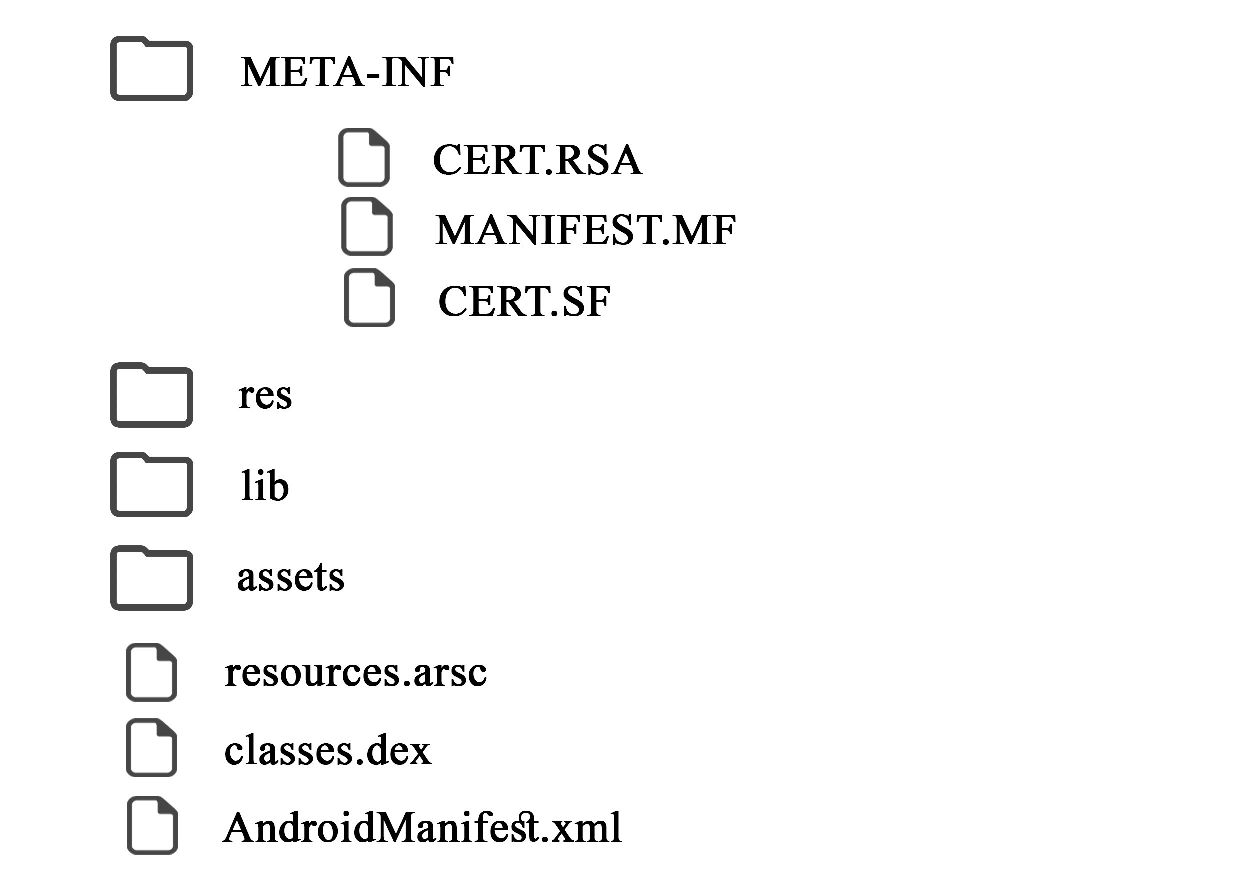
\includegraphics[width=60mm]{images/apkStructure.pdf}
  \end{center}
  \caption{Typická štruktúra APK súboru}
  \label{fig:strukturaApk}
\end{figure}


V APK súbore nájdeme nasledujúce súbory a adresáre:
\begin{itemize}

	\item \bod{AndroidManifest.xml} -- súbor obsahujúci meta informácie o aplikácii. Pomocou tohto súboru oznamuje aplikácia operačnému systému svoju identitu a požiadavky. Android Manifest sa v APK balíčku nachádza vo formáte skompilovaného binárneho XML.
Súbor AndroidManifest.xml obsahuje okrem iného informácie o nasledujúcich vlastnostiach aplikácie:
		
		\begin{itemize}
			\item meno balíku aplikácie slúžiace ako unikátny identifikátor aplikácie,
			\item najnižšiu verziu Android API na ktorej je aplikácia spustiteľná
			\item popisuje základné komponenty aplikácie, obsahuje informácie o aktivitách, službách (service), poskytovateľoch obsahu (content provider), prijímačoch (broadcast receiver) a triedach ktoré ich v rámci aplikácie implementujú,
			\item deklaruje povolenia vyžadované aplikáciou na prístup k zabezpečeným častiam Android API,
			\item definuje povolenia vyžadované od iných aplikácií pri interakcii s danou aplikáciou~\cite{Manifest}.
		\end{itemize}
	
	\item \bod{Classes.dex} -- súbor obsahujúci spustiteľný kód aplikácie. Súbor typu DEX (Dalvik Executable) obsahuje operačné kódy a inštrukcie špecifické pre behové prostredie Android Runtime a virtuálny stroj Dalvik Virtual Machine (pre verzie Android 4.4.4 a staršie)~\cite{DexFormat}. 

	\item \bod{Resources.arsc} -- tento súbor obsahuje informácie o zdrojových súboroch aplikácie. Tento súbor určuje vzťah medzi zdrojovými súbormi a ich identifikátormi, pomocou ktorých sú súbory referencované v zdrojovom kóde aplikácie.
	
	\item \bod{Assets} -- adresár obsahujúci neskomprimované zdrojové súbory.  Na rozdiel od zdrojových súborov z priečinku res, tieto zdroje nie sú referencované identifikátorom, ale prístup k nim je umožnený pomocou API triedy AssetManager.
	
	\item \bod{Lib} -- v tomto adresári sa nachádzajú skompilované knižnice určené pre konkrétnu architektúru procesora. Medzi podporované architektúry patrí ARMv7 a novšie, x86, x86\_64.

	\item \bod{Res} -- adresár obsahujúci zdroje aplikácie. Obsah tohto adresára je tvorený predovšetkým multimediálnymi súbormi ako napríklad obrázky a ikony, ale aj súbormi vo formáte XML ktoré definujú užívateľské rozhranie, farby, lokalizované texty alebo štýl aplikácie. Súbory umiestnené v tomto adresári sú v zdrojovom kóde referencované pomocou unikátnych číselných identifikátorov, ktoré sú vygenerovaný počas kompilácie a nachádzajú sa v triede \zv{R.java}. Obsah priečinku je ďalej logicky členený do viacerých podpriečinkov. Android podporuje lokalizáciu a rôzne verzie zdrojových súborov, ktoré použije na základe údajov o zariadení na ktorom je aplikácia spustená~\cite{Resources}.
	
	\item \bod{META-INF} -- v tomto adresári sa nachádzajú súbory zaručujúce digitálny podpis a integritu APK balíčku. 
		\begin{itemize}
			\item CERT.RSA  -- súbor obsahujúci certifikát podpisu aplikácie
			\item MANIFEST.MF  -- súbor obsahujúci hash každého súboru v APK archíve. Využíva hashovaciu funkciu \zv{SHA-1}.
			\item CERT.SF  -- súbor obsahujúci záznam o každom súbore v APK archíve. Záznam o jednom súbore obsahuje jeho názov a \zv{SHA-1} hash záznamu o tomto súbore z MANIFEST.MF.
		\end{itemize}		
		
		
\end{itemize} 


\section{Distribúcia aplikácií}
Aplikácie na platforme Android sú distribuované ako inštalačné APK balíčky. 

Podľa formy distribúcie a inštalácie môžeme aplikácie rozdeliť na dve základné skupiny
\begin{itemize}
 \item \bod{Predinštalované (systémové) aplikácie} -- tieto aplikácie sú distribuované priamo so zariadením a sú nainštalované pri iniciálnom zapnutí zariadenia,
 \item \bod{Užívateľské aplikácie} -- aplikácie distribuované vo forme balíčkov poskytovaných najčastejšie pomocou obchodov s aplikáciami.
\end{itemize}

Zoznam predinštalovaných aplikácií určuje výrobca zariadenia. Používateľ nemá možnosť systémové aplikácie odinštalovať. Do kategórie predinštalovaných systémových aplikácií patria aplikácie umožňujúce ovládanie základného vybavenia zariadenia ako napríklad aplikácia telefón alebo fotoaparát. Do tejto kategórie patria aj predinštalované služby od spoločnosti Google. 

Užívateľské aplikácie slúžia na prispôsobenie systému pre potreby konkrétneho užívateľa. O inštalácií a odstránení užívateľských aplikácií rozhoduje používateľ. Na pohodlné prehliadanie a inštaláciu aplikácií slúžia obchody (app stores). Pomocou centralizovaných obchodov s aplikáciami môžu softvéroví vývojári jednoducho dostať svoju aplikáciu k veľkému počtu užívateľov.  Najrozšírenejším a najznámejším obchodom s aplikáciami pre platformu Android je oficiálny obchod 
\zv{Google Play Store}. 

Okrem oficiálneho obchodu sú aplikácie distribuované aj pomocou alternatívnych distribučných kanálov. Medzi takéto kanály zaraďujeme alternatívne obchody s aplikáciami ako napríklad \zv{Amazon Appstore}. Častým distribučným kanálom sú aj obchody výrobcov mobilných zariadení alebo obchody mobilných operátorov. Existuje viacero služieb tretích strán ktoré sprostredkovávajú prístup k oficiálnym aplikáciám z týchto obchodov. APK súbory sú distribuované aj pomocou warezových portálov na zdieľanie súborov alebo underground obchodov. 

Z dôvodu udržania bezpečného a spoľahlivého fungovania platformy Android je dôležitá bezpečnosť a kvalita distribuovaných aplikácií. Výskum porovnávajúci kvalitu aplikácií na neoficiálnych distribučných platformách ukázal, že tieto distribučné kanály obsahujú $5 až 13\%$ aplikácií, ktoré sú klonom oficiálnych aplikácií distribuovaných pomocou \zv{Google Play Store} ~\cite{Zhou2012}.

\section{Inštalácia aplikácií}

Platforma Android poskytuje služby na inštaláciu, aktualizáciu a odinštalovanie aplikácií. \newline
Základnú funkcionalitu poskytujú nasledujúce služby.
\begin{itemize}
	\item \bod{Package Installer} -- implementuje funkcionalitu inštalácie, aktualizácie a odinštalovania aplikácií,
	\item \bod{Package Manager Service} -- poskytuje API pre správu nainštalovaných softvérových balíčkov,
	\item \bod{Daemon Installd} -- vytvára a spravuje adresáre potrebné pre nainštalovanie aplikácie.
\end{itemize}
Inštalácia aplikácie pozostáva z overenia aplikácie a extrakcie dát z APK balíčka. Aplikácia je overená na základe digitálneho podpisu a metadát zo súboru \zv{AndroidManifest.xml}. Systémové aplikácie sú rozbalené do adresára \cesta{/system/app}. Užívateľské aplikácie sú nainštalované v adresári \cesta{/data/app}. Systém Android uchováva v spomínaných adresároch kompletné APK súbory~\cite{AndroidDeveloper}.

\section{Bezpečnosť}

Bezpečnosť a integrita distribuovaných APK balíčkov je dôležitým aspektom zabezpečenia celého systému Android.

\subsection{Podpis aplikácie}

Každý APK balíček musí byť digitálne podpísaný. Systém Android zabráni inštalácii digitálne nepodpísaných aplikácií. 
Súbory súvisiace s podpisom APK balíčku sa nachádzajú v priečinku \zv{META-INF}. Počas digitálneho podpisu aplikačného balíčku sa vygenerujú \zv{SHA-1} alebo \zv{SHA-256} hashe súborov obsiahnutých v APK archíve. Záznamy o súboroch a ich hashoch sú uložené v súboroch \cesta{META-INF/MANIFEST.MF} a \cesta{META-INF/CERT.SF}. Celý APK balíček je následne podpísaný pomocou utility \zv{Jarsigner}. 

Android podporuje dve schémy digitálneho podpisu aplikácie. Schéma verzie 1 je založená na podpise štandardného Java balíčka. Táto schéma nechráni niektoré súbory špecifické pre APK balíčky, ako napríklad metadáta o aplikácií. Nechránené súbory musia byť za účelom overenia dekomprimované počas procesu overenia, čo zvyšuje časovú a pamäťovú náročnosť overenia APK balíčku.  Od verzie \zv{Android 7.0} (verzia API 24) je podporovaná schéma podpisu vo verzii 2, ktorá je upravená a špecializovaná na podpis APK balíčka a eliminuje nedostatky verzie 1. V súčasnosti sú aplikácie zvyčajne podpísané obidvomi spôsobmi~\cite{NT0FrzQIkOAYbG2Ga}.
\newline \newline
\noindent \textbf{Kontrola integrity} \newline \newline
\noindent Hashe jednotlivých súborov v APK balíčku vygenerované počas procesu podpisu, slúžia na zaručenie integrity. Počas inštalácie aplikácie sa v rámci procesu overenia aplikácie kontrolujú hashe jednotlivých súborov. V prípade zmeny súborov v aplikácií bez jej opätovného podpisu, systém zabráni inštalácií. Pri zmene obsahu musí byť APK balíček podpísaný znova. 
\newline \newline
\noindent \textbf{Identifikácia autora} \newline \newline
\noindent Podpis balíčka slúži na identifikáciu autora aplikácie. V prípade, že je viacero aplikácií podpísaných jedným kľúčom, pochádzajú tieto aplikácie od jedného vydavateľa. 
Všetky verzie jednej aplikácie musia byť podpísané rovnakým certifikátom. Unikátnym identifikátorom aplikácie je meno hlavného balíka aplikácie (package name). Android považuje aplikácie s rovnakým menom balíka za rôzne verzie jednej aplikácie a pri aktualizácií nahrádza staršiu verzie novšou. Všetky aplikácie s rovnakým menom balíka musia byť preto podpísané rovnakým certifikátom, čo zaručuje, že pochádzajú od rovnakého vydavateľa.  V prípade, že sú podpísané rôznymi certifikátmi, Android ich inštaláciu zamietne. 
\newline \newline
\noindent \textbf{Správa podpisových kľúčov} \newline \newline
\noindent Platforma Android povoľuje používanie tzv. \zv{self-signed} certifikátov. \zv{Self-signed} certifikáty sú podpísané identitou ktorú identifikujú. 

Z pohľadu vývojára je správa podpisového kľúča veľmi dôležitá. Vývojári aplikácií majú pri správe podpisového kľúča dve možnosti. Môžu používať manuálnu správu, alebo službu \zv{Google Play App Signing}. 
\begin{itemize}
	\item \bod{Manuálna správa kľúča} -- v prípade použitia manuálnej správy kľúča je aplikácia podpísaná vývojárom a nahraná do obchodu s aplikáciami. Z tadiaľ je ďalej distribuovaná k užívateľom. V prípade straty podpisového kľúča nie je vývojár aplikácie schopný vydávať nové verzie aplikácie pod rovnakým názvom balíku.
	\item \bod{Google Play App Signing} -- pri použití bezpečnej správy podpisových kľúčov \zv{Google Play App Signing} je kľúč používaný na podpis balíčka spravovaný službou  \zv{Google Play}. Vývojár podpíše aplikáciu svojim kľúčom používaným na komunikáciu so službou  \zv{Google Play}, ktorá aplikáciu na novo podpíše podpisovým kľúčom. Aplikácia distribuovaná k užívateľom je teda podpísaná kľúčom, ktorý je manažovaný službou \zv{Google Play}~\cite{NT0FrzQIkOAYbG2G}. 
\end{itemize}


\subsection{Známe bezpečnostné riziká}

Existuje viacero známych zraniteľností súvisiacich s distribúciou aplikácií  pre platformu Android. Najviac rozšíreným problémom je prebaľovanie APK balíčkov. Pri tomto procese je aplikácia rozbalená a niektoré časti aplikácie sú upravené. Modifikovaná aplikácia je ďalej distribuovaná. Detailný popis prebaľovania aplikácií a rizík s tým spojených sa nachádza v kapitole TODO.

Metóda prebaľovania upraví aplikáciu a na novo ju podpíše iným podpisovým kľúčom. Ďalšie známe metódy útokov využívajú predovšetkým zraniteľnosti pri overovacom procese APK balíčku a nemodifikujú originálny podpis. 

Zraniteľnosť pri inštalácií nekompletného APK súboru využíva fakt, že pri overovaní hashov súborov sa ignorujú záznamy, ktoré v balíku neexistujú. Súbory je teda možné z APK archívu odstrániť bez jeho opätovného podpísania. Modifikovanú aplikáciu je možné distribuovať ako originálnu verziu. Aplikácia po odstránení súborov nebude pracovať správne a môže dostať celé zariadenia do nepoužiteľného stavu~\cite{A7idcou1z6WqKvQZ}.

Pri verifikačnom procese sa nekontrolujú súbory slúžiace na podpis balíčka. To umožňuje útočníkovi nahrať do adresára \zv{META-INF} ľubovoľný súbor bez potreby opätovného podpísania. Útočník tak môže do aplikácií nahrať kusy kódu. Tento kód však nevykoná pôvodná aplikácia, ktorej zdrojové kódy zostali nepozmenené. Namiesto toho útočník distribuuje svoju vlastnú aplikáciu, ktorá pomocou classloaderu použije daný kód vložený do originálnej aplikácie~\cite{A7idcou1z6WqKvQZ}.

% Repackaging
\chapter{Prebalené aplikácie}
\label{chap:repackaging}
Prebaľovanie aplikácií je formou útoku na systému Android. Princíp útoku spočíva v~modifikácii originálnej aplikácie a jej následnej redistribúcii. Počas modifikácie APK súboru môže útočník pridať škodlivú funkcionalitu a upraviť tak správanie aplikácie.
Prebaľovanie aplikácií je jednou z~najbežnejších techník distribúcie malvéru a škodlivého kódu na platforme Android. 

Štandardný postup tvorby prebalených aplikácií z~pohľadu útočníka:
\begin{enumerate}
	\item Stiahnutie populárnej aplikácie,
	\item Dekompilácia aplikácie pomocou nástrojov reverzného inžinierstva,
	\item Modifikácia aplikácie pridaním škodlivého kódu,
	\item Zabalenie aplikácie,
	\item Podpísanie vlastným self-signed certifikátom,
	\item Distribúcia aplikácie pomocou oficiálnych a neoficiálnych kanálov.
\end{enumerate}

Tvorcovia prebalených aplikácií využívajú popularitu originálnych aplikácií za účelom propagácie malvéru. Cieľom prebaľovania APK súborov nie je vytvoriť novú odlišnú aplikáciu s~využitím zdrojového kódu a vlastností existujúcej aplikácie. Namiesto toho je zámerom prebalených aplikácií vydávať sa za pôvodnú aplikáciu a pripomínať ju v~maximálnej možnej miere. Modifikované verzie navonok pôsobia identicky ako originálne verzie. Z~pohľadu užívateľa poskytuje modifikovaná aplikácia rovnakú funkcionalitu a užívateľské rozhranie ako originál~\cite{Chen2015,plagScaleable}. 

Prebaľovanie aplikácií je populárne aj vďaka warezovým portálom slúžiacich na zdieľanie nelegálneho obsahu. Warezové portály ponúkajú bezplatne aj aplikácie, ktoré sú v~službe \zv{Google Play} dostupné iba za poplatok, čo výrazne prispieva k~šíreniu takýchto aplikácií. Prebalené aplikácie však nie sú distribuované výhradne pomocou neoficiálnych kanálov, ale aj prostredníctvom \zv{Google Play}.

Prebalené aplikácie sú škodlivé nie len pre koncových užívateľov, ale aj vývojárov, vlastníkov duševných práv a prevádzkovateľov obchodov s~aplikáciami~\cite{CloneRelative}. 

\section{Spôsob modifikácie aplikácií}
Za účelom modifikácie aplikácie upraví útočník inštalačný APK balíček. Modifikácia už existujúcej nainštalovanej aplikácie nie je možná. Spravidla je modifikovaný len jej inštalačný balíček a škodlivá aplikácia sa do zariadenia dostane inštaláciou takéhoto balíčku.
APK súbory majú definovaný formát a štruktúru, ktoré sú popísané v~kapitole \ref{sec:struktura}. Vďaka ich formátu a štrukturovanému procesu tvorby je ich dekompilácia nenáročná.

Existuje viacero nástrojov reverzného inžinierstva, ktoré môžu byť použité pri tvorbe prebalených aplikácií. Najkomplexnejším nástrojom, ktorý je možné použiť na kompletné rozbalenie a následné zabalenie aplikácie je nástroj ApkTool~\cite{Apktool}. Za účelom modifikácie zdrojového kódu je možné využiť bežne dostupné nástroje ako \zv{dex2jar}, \zv{jd-gui} a \zv{smali} ~\cite{Dex2jar, jdgui, smali}.

Z~hľadiska modifikácie sú pri prebaľovaní zaujímavé nasledujúce súbory:

\begin{itemize}
	\item \bod{AndroidManifest.xml} -- upravením tohto súboru je možné pridávať nové bezpečnostné povolenia. Súbor je v~APK balíku dostupný ako skomprimované XML. Skomprimované (binárne) XML je možné konvertovať do editovatelnej formy pomocou nástroja \zv{ApkTool}~\cite{Apktool}.
	\item \bod{Classes.dex} -- vykonanie zmien v~zdrojovom kóde umožňuje komplentú modifikáciu funkcionality aplikácie. Tento súbor obsahujúci skompilovaný zdrojový kód aplikácie je možné editovať pomocou spomínaných nástrojov \zv{dex2jar}, \zv{jd-gui} a \zv{smali}.
\end{itemize}

Zásadnou vecou, ktorá odlišuje prebalenú aplikáciu od originálu je digitálny podpis. Po editácii aplikácie a jej opätovnom zabalení je nutné aplikáciu digitálne podpísať. Za predpokladu, že privátny kľúč pôvodného vydavateľa neunikol a nie je k~dispozícii útočníkovi, podpis originálnej a prebalenej aplikácie sa bude líšiť~\cite{Nolan2012a}. 

\section{Časté typy modifikácie}

Modifikácia zdrojových kódov aplikácie predstavuje vážne ohrozenie bezpečnosti. Nasledujúce body popisujú najčastejšie typy modifikácie zdrojových kódov.

\subsection*{Modifikácia reklamných modulov}
Väčšina aplikácií je užívateľom dostupná zadarmo. Zdroj príjmu pre vývojárov predstavujú reklamné moduly integrované do aplikácie. Najčastejšou modifikáciou vykonávanou pri prebaľovaní aplikácií je nahradenie pôvodných reklamných modulov. Výnosy z~reklamy sú tak presmerované z~účtu pôvodného vývojára na účet útočníka. Najjednoduchšou úpravou je využitie existujúcich reklamných služieb a presmerovanie zisku na iný účet pomocou zmeny API kľúča. Takmer 65 \% prebalených aplikácií obsahuje modifikované reklamné knižnice~\cite{fakeapps}.

\subsection*{Zneužitie prémiových služieb}
Niektoré prebalené aplikácie obsahujú platené služby, ktoré nie sú súčasťou originálnej aplikácie. Najčastejším spôsobom zneužitia prémiových služieb je odosielanie textových správ na spoplatnené prémiové čísla. Prebalená aplikácia vyžaduje pri inštalácii povolenie na odosielanie správ, ktoré ďalej odosiela bez používateľovho vedomia. Takto upravená aplikácia môže zaregistrovať vlastnú službu, ktorá odfiltruje SMS správy od telekomunikačného poskytovateľa a zabráni tak upozorneniam o~využití platených prémiových služieb. Známym príkladom takto napadnutej aplikácie je prehliadač QQ Browser~\cite{fakeapps}.

\subsection*{Prístup k~citlivým dátam}
Aplikácie môžu byť upravené za účelom zbierania informácií ako telefónne čísla kontaktov, emailové adresy, história prehliadača alebo zoznam nainštalovaných aplikácií. Túto činnosť vykonávajú služby na pozadí. Zozbierané dáta sú odosielané na vzdialené webové servre. 

\subsection*{Inštalácia malvéru}
Prebalené aplikácie môžu na pozadí spustiť sťahovanie a inštaláciu ďalšieho malvéru. 

\subsection*{Vzdialený prístup a ovládanie zariadenia}
Za účelom získania kontroly nad zariadením môže aplikácia nadviazať spojenie so vzdialeným serverom, ktorý je pod kontrolou útočníka. Server posiela aplikácii príkazy a prijíma od nej odpovede. Príkladom takéhoto správania je prebalená verzia aplikácie Stupid Birds, ktorá obsahuje vložený kód, pomocou ktorého sa pripojí na URL adresu z~ktorej prijíma príkazy. Na základe týchto príkazov dokáže aplikácia na pozadí stiahnúť iné aplikácie, a umiestniť odkazy na ich inštaláciu priamo na plochu zariadenia~\cite{fakeapps}. 

\subsection*{Vloženie viacerých DEX súborov}
Po zmenách aplikácie prezentovaných v~predchádzajúcich bodoch je nutné APK balíček nanovo podpísať. Vo verziách Android 4.4 a nižších existuje zraniteľnosť známa ako Master Key vulnerability. Ide o~jednu z~najzávažnejších zraniteľností pri overovaní APK balíčku počas jeho inštalácie. V~prípade, že APK balíček obsahuje dva súbory s~rovnakým názvom, pri overovaní hashov súborov sa použije prvý záznam o~takomto súbore, avšak Android použije pri inštalácii druhý súbor. To umožňuje upraviť aplikáciu bez potreby opätovného podpísania. Tento fakt je možné využiť na vloženie nového súboru so zdrojovým kódom, ktorý kompletne nahradí pôvodnú logiku alebo vzhľad aplikácie~\cite{Jung2013,c2gYRVCI9leJhfOJ}.

\section{Výskyt prebalených aplikácií}
Pre platformu Android existujú milióny aplikácií. Počet aplikácií dostupných v~oficiálnom obchode \zv{Google Play} prekročil v~septembri 2017 3 milióny~\cite{Statista}. Množstvo aplikácií je dostupných prostredníctvom neoficiálnych distribučných kanálov.  Výsledky predchádzajúcich výskumov ukazujú, že prebalené aplikácie predstavujú nezanedbateľnú časť dostupných aplikácií.

Analýzou 23\,000 aplikácií zo šiestich alternatívnych obchodov v~rámci práce \zv{Detecting Repackaged Smartphone Applications in
Third-Party Android Marketplaces} sa zistilo, že pomer prebalených aplikácií sa v~alternatívnych obchodoch pohybuje medzi 5 až 13 \% ~\cite{DetectingRepackagedZhou}.
Počet aplikácií, ktoré sú nie len prebalené, ale pridávajú do originálnych aplikácií škodlivé správanie je taktiež významný. Wu Zhou a kolektív na základe analýzy vzorky 85\,000 aplikácií identifikovali, že počet takýchto aplikácií sa pohybuje medzi 0,97 až 2,7 \% všetkých aplikácií~\cite{Zhou2013}.
Až 86 \% aplikácií obsahujúcich malvér vzniklo prebalením originálnej aplikácie a vložením škodlivého kódu~\cite{androidThreats}.

Alternatívne distribučné platformy, ktoré často neposkytujú dostatočnú formu kontroly obsahu, obsahujú väčší počet prebalených APK súborov ako oficiálne zdroje~\cite{Zhauniarovich2013}. 

% Zname metody detekcie prebalených aplikácií
\chapter{Známe metódy detekcie prebalených aplikácií}
Šírenie prebalených aplikácií predstavuje významnú hrozbu pre celý systém Android. Z hľadiska bezpečnosti systému je v súčasnosti detekcia prebalených aplikácií jednou z najdôležitejších tém.
Téme prebalených APK súborov sa vo svojich prácach venuje viacero výskumných tímov. Bolo navrhnutých a implementovaných viacero spôsobov detekcie takýchto aplikácií. 
\newline 

\noindent Detekcia prebalených APK balíčkov vychádza z nasledujúcich pozorovaní
\begin{itemize}
	\item Prebalená aplikácia zachováva funkcionalitu pôvodnej aplikácie
	\item Prebalená aplikácia zachováva vzhľad pôvodnej aplikácie
	\item Prebalená a pôvodná aplikácia sú podpísané rôznymi entitami
\end{itemize} 

\noindent Algoritmy detekcie prebalených aplikácií pozostávajú zvyčajne z dvoch základných krokov
\begin{itemize}
	\item Extrakcia vlastností aplikácií
	\item Párové porovnanie aplikácií na základe extrahovaných vlastností
\end{itemize}
\ \newline

\noindent Základným rozdielom medzi existujúcimi metódami detekcie prebalených APK súborov sú vlastnosti aplikácií použité pri detekcii malvérových duplikátov. Väčšia časť existujúcich algoritmov využíva podobnosť zdrojových kódov a inštrukcií. Existuje niekoľko metód, ktoré na detekciu prebalených aplikácií využívajú podobnosť multimediálnych súborov obsiahnutých v APK balíčkoch.

\section{DroidMOSS}
Metóda \zv{DroidMOSS} je založená na podobnosti zdrojového kódu originálu a prebalenej kópie. Táto metóda sa zameriava na podobnosť aplikačného Java kódu a nezaoberá sa natívnym kódom. Počas prebaľovania je jednoduchšie modifikovať Java kód ako natívny kód a len malá časť aplikácií (približne 5 \% používa natívny kód).


\zv{DroidMOSS} pozostáva z troch kľúčových krokov. Prvým krokom je extrakcia aplikačných inštrukcií a získanie informácií o vydavateľovi aplikácie v podobe certifikátu. Tieto dva atribúty charakterizujú a odlišujú aplikácie.
Za účelom extrakcie aplikačného kódu je použitý nástroj \zv{smali/baksmali}, pomocou ktorého je súbor \zv{classes.dex} dekompilovaný do Dalvik bytekódu~\cite{smali}.  Počas procesu prebaľovania môže byť použitá obfuskácia kódu. Počas obfuskácie sú premenované názvy balíkov, tried, metód a premenných. \zv{DroidMOSS} sa s obfuskáciou kódu vysporiadava pomocou ignorovania operandov. Pri tvorbe identifikátora aplikácie sú zohľadnené len operačné inštrukcie. Intuitívne môžeme tento prístup vysvetliť tak, že počas prebaľovania je jednoduché upraviť kód premenovaním premenných, oveľa náročnejšie je zmeniť kód tak, aby používal odlišné inštrukcie. 
Informácie o autorovi aplikácie pochádzajú zo súborov v adresári \cesta{META-INF}. \zv{DroidMOSS} vygeneruje identifikátor autora pomocou zahashovania verejného kľuča, mena vývojára a jeho kontaktných informácií. 


Druhý krok spočíva vo vygenerovaní unikátneho identifikátoru každej aplikácie. Hlavným dôvodom pre tvorbu identifikátoru je komplexnosť a veľký počet inštrukcií v jednej aplikácií. Dĺžka identifikátoru je výrazne kratšia ako dáta o inštrukciách aplikácie, čo umožňuje efektívnejšie porovnávanie aplikácií. 
Vytvorenie identifikátoru pomocou hashovania celého kódu aplikácie môže byť efektívne použité na overenie úplnej zhody dvoch aplikácií. Tento postup však nie je možné aplikovať pri určení podobnosti aplikácií.  Z tohto dôvodu využíva \zv{DroidMOSS} špeciálnu hashovaciu techniku \zv{fuzzy hashing} \cite{fuzzyHashing}. Namiesto vytvorenia identifikátoru celej sekvencie inštrukcií, je táto sekvencia najprv rozdelená na kratšie časti. Následne je každá z týchto častí hashovaná osobitne. Na vyhodnotenie podobnosti aplikácií sú použité identifikátory (hashe) týchto kratších sekvencií.


Posledným krokom je párové porovnanie aplikácií. Aplikácie sú  rozdelené do dvoch skupín. Jedna skupina obsahuje aplikácie z \zv{Google Play Store}, druhá aplikácie z neoficiálnych zdrojov.  \zv{DroidMOSS} využíva silný predpoklad, že aplikácie pochádzajúce z \zv{Google Play Store} nie sú prebalené. 
Aplikácie z rozdielnych skupín sú vzájomne porovnané. Na vyhodnotenie podobnosti je použitý algoritmus navrhnutý pomocou techniky dynamického programovania. Podobnosť aplikácií je určená ako minimálna vzdialenosť medzi identifikátormi dvoch sekvencii inštrukcií.  Vzdialenosť je reprezentovaná počtom úprav potrebných na pretvorenie identifikátora jednej sekvencie na identifikátor druhej sekvencie. Ak vypočítaná podobnosť presiahne definovanú hranicu a porovnávané aplikácie sú podpísané rôznymi vydavateľmi, aplikácia ktorá nepochádza z \zv{Google Play Store} je označená za prebalenú. Použitá technika umožňuje efektívne lokalizovať zmeny vykonané v prebalených aplikáciách. 

\begin{figure}[htb]
  \begin{center}
    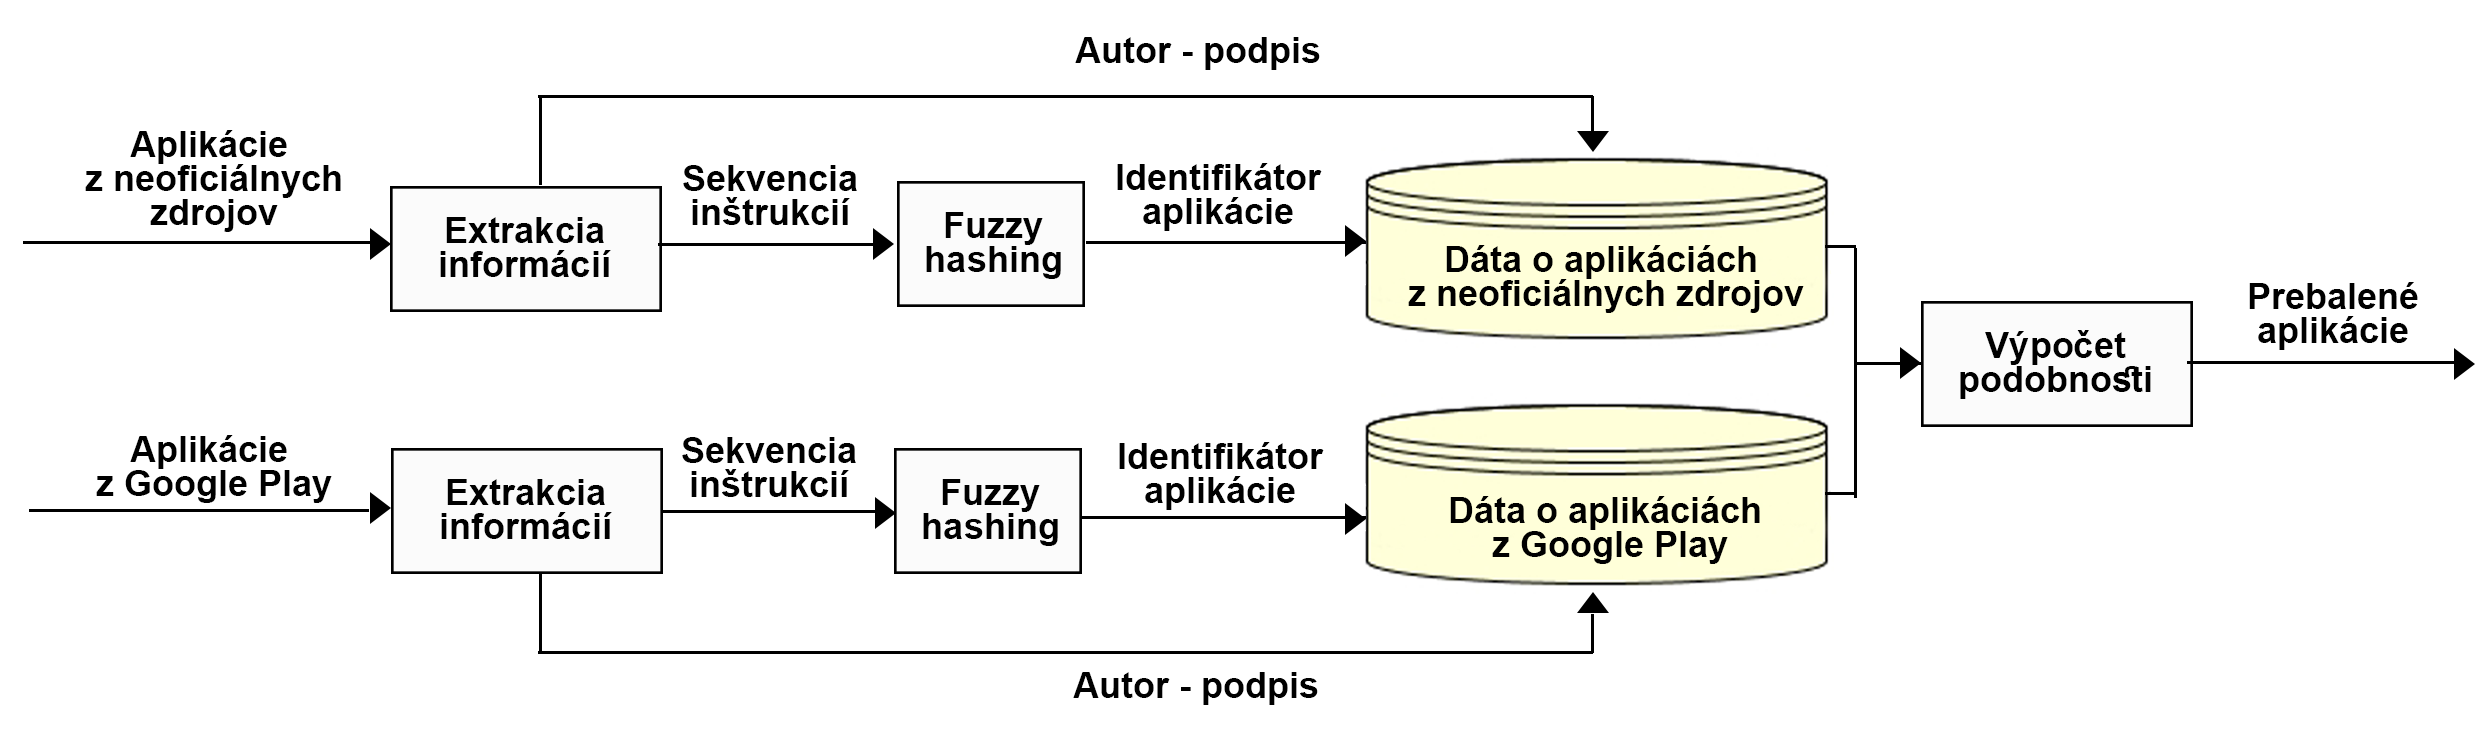
\includegraphics[width=130mm]{images/DroidMoss.png}
  \end{center}
  \caption{Postup metódy DroidMOSS}
  \label{fig:strukturaApk}
\end{figure}


Systém \zv{DroidMOSS} bol aplikovaný na kolekciu $86\,000$ aplikácií. Pomocou tejto techniky sa ukázalo, že $5$ až $13\%$  aplikácií distribuovaných pomocou alternatívnych zdrojov je prebalených~\cite{DetectingRepackagedZhou}.


\section{ImageStruct}
Metóda \zv{ImageStruct} používa pri detekcii prebalených aplikácií podobnosť obrázkových súborov. Tento spôsob je založený na pozorovaní, že podobné aplikácie (rôzne verzie tej istej aplikácie alebo prebalené aplikácie) obsahujú podobné obrázky, zatiaľ čo obrázky v aplikáciách s rôznou funkcionalitou sú rozdielne. 


\zv{ImageStruct} získava z APK balíčka charakteristické dáta obrázkov. Na extrakciu obrázkových dát je použitý algoritmus \zv{pHash}. \zv{PHash} používa diskrétnu kosínusovú transformáciou, pomocou ktorej z obrázka odstráni niektoré farebné frekvencie. To umožňuje detekciu podobnosti aj pri jednoduchších úpravách, ako napríklad zmena rozlíšenia alebo vystrihnutie časti obrazu~\cite{pHash}. Na identifikáciu vydavateľa sú použité údaje z priečinka \cesta{META-INF}.


Extrahované dáta sú ukladané v databáze \zv{Redis}, ktorá slúži ako rýchla cache pamäť. 
Podobnosť dvoch APK súborov je určená ako pomer spoločných obrázkov a všetkých obrázkov jednej z aplikácií. Na výpočet podobnosti sa používa formula:
\[ similarity(app_1, app_2) = \frac{|app_{1}images \cap app_{2}images|} { app_{1}images} \]


\zv{ImageStruct}  porovnáva kolekciu aplikácií z \zv{Google Play} s aplikáciami z alternatívnych obchodov, pričom využíva predpoklad, že \zv{Google Play} neobsahuje prebalené aplikácie. Ak hodnota podobnosti prekročí stanovenú hranicu a aplikácie sú podpísané rôznymi autormi, aplikácia z alternatívneho zdroja je označená za prebalenú.
Nastavenie hodnoty hranice nad ktorou sú aplikácie považované za duplikáty je z hľadiska presnosti a spoľahlivosti detekcie kľúčové. Autori uvádzajú, že pomocou viacerých experimentov určili túto hodnotu na $0,6$~\cite{ImageStruct}.

\begin{figure}[htb]
  \begin{center}
    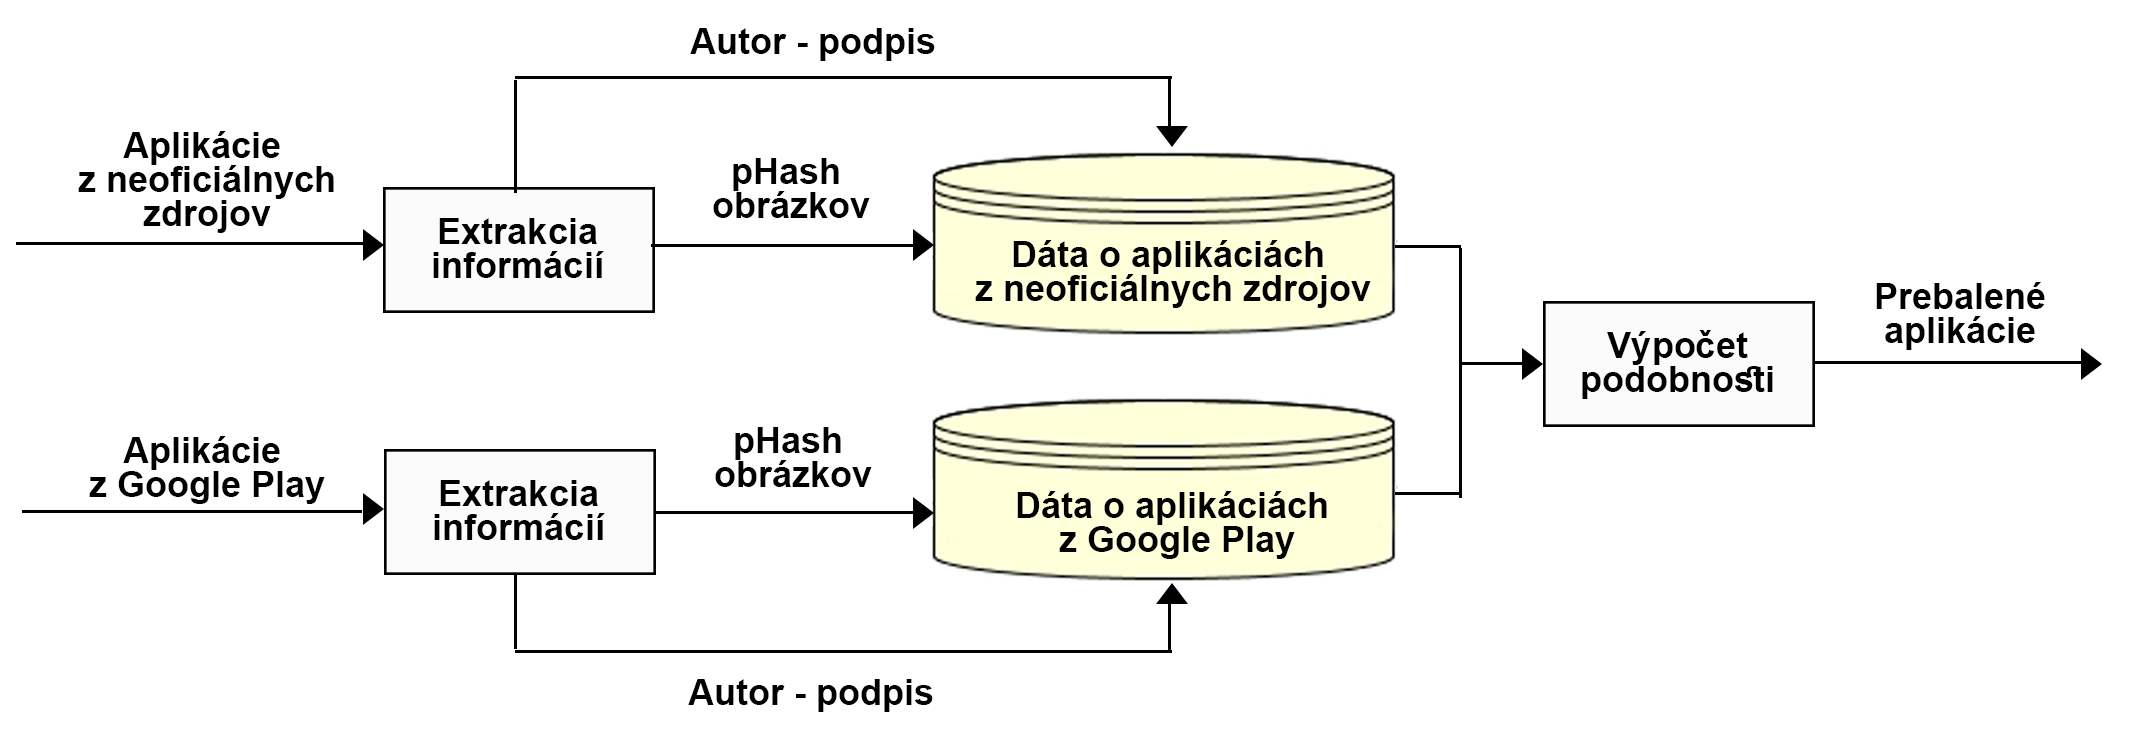
\includegraphics[width=130mm]{images/ImageStruct.png}
  \end{center}
  \caption{Postup metódy ImageStruct}
  \label{fig:strukturaApk}
\end{figure}

Pomocou experimentov nad databázou $48\,000$ aplikácií z \zv{Google Play} a alternatívnych zdrojov odhalila táto metóda, že výskyt prebalených aplikácií v alternatívnych zdrojoch sa pohybuje medzi $6,7 \%$ až $14.5 \%$.
Pomer prebalených aplikácií detekovaných touto metódou je takmer rovnaký ako v prípade metódy \zv{DroidMOSS}. Ako dôkaz použiteľnosti metód zameraných na podobnosť multimediálnych súborov bolo v rámci experimentov vykonané porovnanie hodnôt podobnosti určených metódou \zv{ImageStruct} a metódou \zv{AndroGuard}, ktorá využíva podobnosť zdrojového kódu. Výsledky ukazujú, že medzi týmito postupmi existuje silná korelácia~\cite{ImageStruct}. 

% Zaver
\chapter{Záver}
Táto diplomová práca sa zaoberala možnosťami analýzy nainštalovaných aplikácií na zariadeniach s operačným systémom Android. Práca sa zameriavala predovšetkým na získavanie metadát o aplikáciách a ich využití pri detekcii prebalených aplikácií.

Primárny cieľom práce bolo vytvorenie softvérového riešenia na detekciu prebalených aplikácií pre mobilný operačný systém Android. Cieľom práce bolo sprístupniť metódu detekcie potenciálne škodlivých aplikácií užívateľom prostredníctvom mobilnej aplikácie, ktorá poskytuje detailné informácie o nainštalovaných aplikačných balíčkoch.  
Za účelom dosiahnutia tohto cieľa sa táto práca zaoberala dvomi hlavnými témami. Prvou z nich bol vývoj mobilnej aplikácie, ktorá získava metadáta o ostatných aplikáciách. Druhú tému predstavuje návrh a implementácia metódy detekcie prebalených aplikácií. 

V rámci tejto práce bola vyvinutá mobilná aplikácia \zv{Apk Analyzer}. Táto aplikácia poskytuje užívateľovi detailné informácie o aplikačných balíčkoch nainštalovaných na jeho zariadení. Na rozdiel od ostatných dostupných aplikácií ponúkajúcich podobnú funkcionalitu, umožňuje naša aplikácia analýzu APK súborov, ktoré nie sú nainštalované. \zv{Apk Analyzer}taktiež zobrazuje detaily dezpečnostných povolení a zoznamy aplikácií, ktoré dané povolenia vyžadujú. Aplikácia umožňuje užívateľom získať prehľad o základných štatistických informáciách o kolekcii aplikácií nainštalovaných na ich zariadení. Aplikácia taktiež poskytuje zrozumiteľné vysvetlenie prezentovaných dát a ponúka užívateľom možnosť detekcie prebalených APK súborov.  Aplikácia \zv{Apk Analyzer} (\zv{sk.styk.martin.apkanalyzer}) je dostupná prostredníctvom obchodu \zv{Google Play}. Od prvého vydania aplikácie v októbri 2017 si ju nainštalovalo viac ako 20\,000 (TODO) užívateľov. Kvalitu aplikácie dokumentuje jej hodnotenie v službe \zv{Google Play}. Aplikáciu v odbobí do marca 2018 ohodnotilo 165 užívateľov a dosiahla priemerné hodnotenie 4,7 hviezdičiek (maximum je 5) (TODO update).

V práci bola navrhnutá nová metóda detekcie prebalených aplikácií. Metóda je založená na základoch aktuálnych poznatkov, ktoré odhaľujú, že pri prebaľovaní zvyčajne zostávajú zdrojové súbory nezmenené. Navrhnutá metóda identifikuje prebalené aplikácie na základe zhody obrázkových súborov medzi viacerými aplikačnými balíčkami. Na rozdiel od väčšiny existujúcich prístupov je naša metóda schopná identifikovať, ktorá z aplikácií je originálna a ktoré sú prebalené kópie. Táto metóda pracuje s dynamicky sa vyvíjajúcou databázou metadát o aplikáciách. Na tvorbe tejto databázy sa podieľajú užívatelia mobilnej aplikácie \zv{Apk Analyzer}. Po schválení užívateľom odošle mobilná aplikácia metadáta o všetkých užívateľkých aplikáciách prítomných na danom zariadení. Navrhnutá metóda detekcie prebalených APK súborov bola prakticky implementovaná a nasadená v produkčnom prostredí systému \zv{Apk Analyzer}.
Vytvorená databáza obsahujúca všetky metadáta obsahuje údaje o viac ako 150\,000 aplikáciách. Počas reálneho nasadenia metódy detekcie prebalených súborov bolo identifikovaných niekoľko skutočností, ktoré môžu negatívne ovplyvniť výsledok detekcie, napríklad aplikácie využívajúce minimum vlastných obrázkov, obrázky pochádzajúce z často sa vyskytujúcich knižníc alebo jednoduchá modifikácia obrázkových súborov, ktorá môže detekciu znemožniť. Napriek týmto limitáciám má implementovaná metóda potenciál na odhalenie prebalených aplikácií. Od svojho spustenia v TODO zaznamenala TODO požiadavkov na detekciu prebalených aplikácií, z toho TODO aplikácií bolo vyhodnotených ako nebezpečné.

Spojením mobilnej aplikácie a serverovej časti vzniklo softvérové riešenie, umožňujúce detekciu prebalených aplikácií priamo v Android zariadení. Obidve tieto časti boli nasadené v produkčnom prostredí a sú dostupné užívateľom. Zdrojový kód aplikácií vytvorených v rámci tejto práce je voľne prístupný.

{\csname captions\languagename\endcsname %% Temporarily override
%% the BibLaTeX localization with the original babel definitions.
\makeatletter %% Use the correct localization of the quotations.
  \thesis@selectLocale{\thesis@locale}\makeatother
\printbibliography[heading=bibintoc]} %% Print the bibliography.


%\makeatletter\thesis@blocks@clear\makeatother
%\phantomsection %% Print the index and insert it into the
%\addcontentsline{toc}{chapter}{\indexname} %% table of contents.
%\printindex

\appendix %% Start the appendices.

\end{document}
